\section{Data model and problem}
\label{sec:background}
In this section, we review the principles of general-purpose topic modeling with \lda~\cite{lda}, \tmlda~\cite{DBLP:conf/kdd/WangAB12} and \atam~\cite{atam2}.
\subsection{Mapping Tweets to Documents}
\begin{table}[b!]
\centering
\caption{Mapping tweets to documents}
\label{tab:model:terms}
\begin{tabular}{|c|c|}
\hline
{\bf Term} & {\bf Description}\\
\hline
$\mf P$ & posts\\
\hline
$\mf G$ & regions\\
\hline
$\mf T$ & time periods\\
\hline
$\mf P_g^t$ & posts from region $g$ during time $t$\\
\hline
$D_g^t$ & document-set built by mapping the content\\
& of each post $p\in \mf P_g^t$ to a document\\
\hline
\end{tabular}
\end{table}
By using suitable  geographic granularity (country, state, county) and temporal granularity (week, bi-week and months), we build our document sets  $D_g^t$.
Table~\ref{tab:model:terms} presents a summarized
version of the terminology associated to our work.

% 	\subsection{Uncovering Latent Topics in Tweets}
% 	We now review the principles of general-purpose topic modeling and
% 	health-related topic modeling.
% 	\subsubsection{Uncovering Latent Topics with LDA}
% 	While LDA is successful at uncovering generic topics, its limitations at discovering
% 	infrequent and specific topics such as health has already been shown \cite{atam2,prier2011identifying}.
% 	\subsubsection{General-purpose topic modeling over time with \tmlda}
% 	In ~\cite{DBLP:conf/kdd/WangAB12}, the authors introduce a modified version of the
% 	LDA to take into account the evolution of topics with time.
% 	While being quite elegant in modeling general-purpose topics \tmlda
% 	not specialized to capture \texttt{\emph{health}} transitions over time.
% 	\subsubsection{Uncovering Health Topics with \atam}
% 	The probabilistic \emph{Ailment Topic Aspect Model} was designed 
% 	specifically to uncover latent health-related topics present in a 
% 	collection of tweets~\cite{atam2}. The proposed method achieves
% 	remarkable improvement over LDA in discovering topics that correspond to 
% 	ailments (in addition to discovering general topics).
% 	The topic distribution vector for a sample tweet is shown 
% 	in Figure~\ref{fig:ldavsatam}. Note the stronger relevance to 
% 	health--related matters in this vector than in the topic distribution vector 
% 	generated by LDA for the same tweet. While \atam is effective at modeling health-related topics, 
% 	it is not designed to model topic transitions over time.

\subsection{\lda, \tmlda and \atam}
While LDA is successful at uncovering generic topics, its limitations at discovering
infrequent and specific topics such as health has already been shown \cite{atam2,prier2011identifying}.
In ~\cite{DBLP:conf/kdd/WangAB12}, the authors introduce a modified version of the
LDA to take into account the evolution of topics with time.
While being quite elegant in modeling general-purpose topics \tmlda
not specialized to capture \texttt{\emph{health}} transitions over time.
The probabilistic \emph{Ailment Topic Aspect Model} was designed 
specifically to uncover latent health-related topics present in a 
collection of tweets~\cite{atam2}. The proposed method achieves
remarkable improvement over LDA in discovering topics that correspond to 
ailments (in addition to discovering general topics).
The topic distribution vector for a sample tweet is shown 
in Figure~\ref{fig:ldavsatam}. Note the stronger relevance to 
health--related matters in this vector than in the topic distribution vector 
generated by LDA for the same tweet. While \atam is effective at modeling health-related topics, 
it is not designed to model topic transitions over time. 
\begin{figure}[t!]
\centering
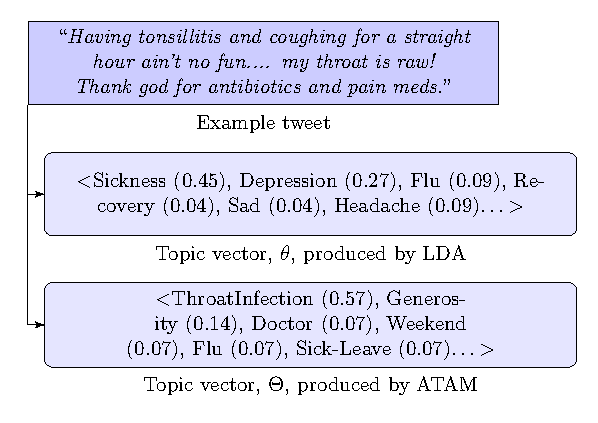
\includegraphics[width=0.45\textwidth]{tikz/exampleTweet1.pdf}
\caption{\lda vs \atam: Comparison of topic distributions for an example tweet.}
\label{fig:ldavsatam}
\end{figure}
\subsubsection{Health Topic Evolution Over Time}
\begin{figure}[b!]
\centering
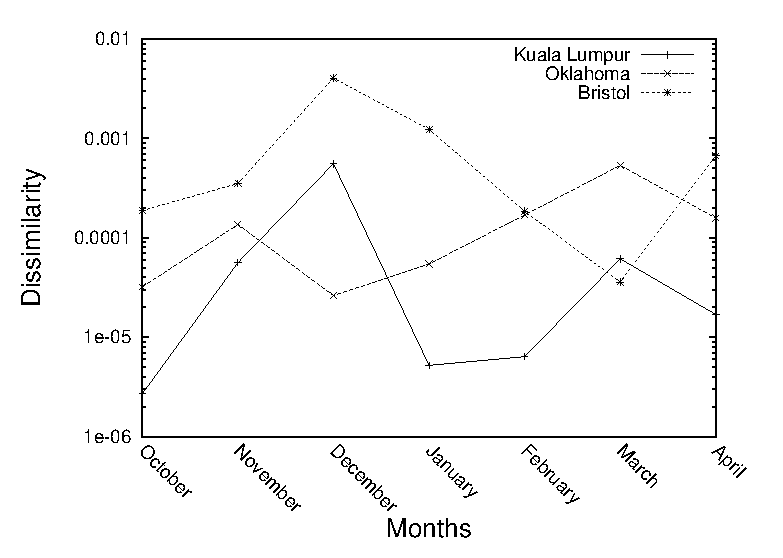
\includegraphics[width=0.45\textwidth]{gnuplot/distributiondifference/bhattacharyadistance.eps}
\caption{Topic transitions over time.}
\label{fig:ailmentsEvolve}
\end{figure}
Let $\Theta_g^t$ be a ailment distribution vector where the weight of each ailment is representative of the discourse density of ailment in the tweets originating from region $g$ during period $t$.
For a region $g$, the interval of time spanning a set of consecutive time periods $\{t_i,t_{i+1},\ldots\}$ during which discovered ailment distributions  $\{\Theta_g^{t_i},\Theta_g^{t_{i+1}},\ldots\}$
do not change appreciably forms a \season w.r.t. ailments. By definition, a \season is (nearly) homogeneous in terms
of ailments. In other words, the ailments evolve in a smooth fashion
within a \season and change abruptly across \season boundary. We posit that such \seasons exist after which they encounter \changes in ailment topic discussions. These \changes in ailment topic discussions 
may be caused by onset of the disease or some other external factors. Nevertheless, they are the interesting points for analyzing purposes.
As an example, in Figure~\ref{fig:ailmentsEvolve}, we show the difference between ailment distributions of consecutive months for 3 different regions Kuala Lumpur (a city in Indonesia), Oklahoma (a state in the USA), and Bristol (a city in the UK). The sharp peaks obtained validate the existence of time intervals that are homogeneous w.r.t. ailments.
